%%% Setup document class.
\documentclass[11pt,]{article}

%%% Setup font.
\usepackage[sc, osf]{mathpazo}

%%% Setup margins.
\usepackage[left = 2cm, right = 2cm, top = 2cm, bottom = 2cm,
includeheadfoot]{geometry}

%%% Setup packages.
\usepackage{multicol}
\usepackage{graphicx}
\usepackage{changepage}
\usepackage{amssymb,amsmath}
\usepackage{ifxetex,ifluatex}
\usepackage{fixltx2e} % provides \textsubscript
\ifnum 0\ifxetex 1\fi\ifluatex 1\fi=0 % if pdftex
  \usepackage[T1]{fontenc}
  \usepackage[utf8]{inputenc}
\else % if luatex or xelatex
  \ifxetex
    \usepackage{mathspec}
  \else
    \usepackage{fontspec}
  \fi
  \defaultfontfeatures{Ligatures=TeX,Scale=MatchLowercase}
\fi
% use upquote if available, for straight quotes in verbatim environments
\IfFileExists{upquote.sty}{\usepackage{upquote}}{}
% use microtype if available
\IfFileExists{microtype.sty}{%
\usepackage{microtype}
\UseMicrotypeSet[protrusion]{basicmath} % disable protrusion for tt fonts
}{}


\setlength{\emergencystretch}{3em}  % prevent overfull lines
\providecommand{\tightlist}{%
  \setlength{\itemsep}{0pt}\setlength{\parskip}{0pt}}
\setcounter{secnumdepth}{0}
% Redefines (sub)paragraphs to behave more like sections
\ifx\paragraph\undefined\else
\let\oldparagraph\paragraph
\renewcommand{\paragraph}[1]{\oldparagraph{#1}\mbox{}}
\fi
\ifx\subparagraph\undefined\else
\let\oldsubparagraph\subparagraph
\renewcommand{\subparagraph}[1]{\oldsubparagraph{#1}\mbox{}}
\fi
\makeatletter
\@ifpackageloaded{caption}{}{\usepackage{caption}}
\AtBeginDocument{%
\ifdefined\contentsname
  \renewcommand*\contentsname{Table of contents}
\else
  \newcommand\contentsname{Table of contents}
\fi
\ifdefined\listfigurename
  \renewcommand*\listfigurename{List of Figures}
\else
  \newcommand\listfigurename{List of Figures}
\fi
\ifdefined\listtablename
  \renewcommand*\listtablename{List of Tables}
\else
  \newcommand\listtablename{List of Tables}
\fi
\ifdefined\figurename
  \renewcommand*\figurename{Figure}
\else
  \newcommand\figurename{Figure}
\fi
\ifdefined\tablename
  \renewcommand*\tablename{Table}
\else
  \newcommand\tablename{Table}
\fi
}
\@ifpackageloaded{float}{}{\usepackage{float}}
\floatstyle{ruled}
\@ifundefined{c@chapter}{\newfloat{codelisting}{h}{lop}}{\newfloat{codelisting}{h}{lop}[chapter]}
\floatname{codelisting}{Listing}
\newcommand*\listoflistings{\listof{codelisting}{List of Listings}}
\makeatother
\makeatletter
\makeatother
\makeatletter
\@ifpackageloaded{caption}{}{\usepackage{caption}}
\@ifpackageloaded{subcaption}{}{\usepackage{subcaption}}
\makeatother

% Custom section fonts
\usepackage{sectsty}
\sectionfont{\rmfamily\mdseries\large\bf}
\subsectionfont{\rmfamily\mdseries\normalsize\scshape}

% Make lists without bullets
\renewenvironment{itemize}{
  \begin{list}{}{
    \setlength{\leftmargin}{1.5em}
  }
}{
  \end{list}
}

% Make parskips rather than indent with lists.
\usepackage{parskip}
\usepackage{titlesec}
\titlespacing\section{0pt}{12pt plus 4pt minus 2pt}{4pt plus 2pt minus 2pt}
\titlespacing\subsection{0pt}{12pt plus 4pt minus 2pt}{4pt plus 2pt minus 2pt}

% Use fontawesome. Note: you'll need TeXLive 2015. Update.
\usepackage{fontawesome}

% Fancyhdr, as I tend to do with these personal documents.
\usepackage{fancyhdr,lastpage}
\pagestyle{fancy}
\renewcommand{\headrulewidth}{0.0pt}
\renewcommand{\footrulewidth}{0.0pt}
\lhead{}
\chead{}
\rhead{}
\lfoot{ \scriptsize \emph{Last update:} \apstylekinda\today }
\cfoot{\scriptsize  Lennart Oelschläger }
\rfoot{\scriptsize \thepage/{\hypersetup{linkcolor=black}\pageref{LastPage}}}

% Always load hyperref last.
\usepackage{hyperref}
\PassOptionsToPackage{usenames,dvipsnames}{color} % color is loaded by hyperref

\hypersetup{unicode=true,
            pdftitle={Lennart Oelschläger:  Curriculum Vitae of Lennart Oelschläger (Curriculum Vitae)},
            pdfauthor={Lennart Oelschläger},
            colorlinks=true,
            linkcolor=blue,
            citecolor=Blue,
            urlcolor=blue,
            breaklinks=true, bookmarks=true}
\urlstyle{same}  % don't use monospace font for urls

%%% Make AP style (kinda) dates for the updated/today field.
\usepackage{datetime}
\newdateformat{apstylekinda}{\shortmonthname[\THEMONTH]. \THEDAY, \THEYEAR}

%%% Start document.
\begin{document}

\begin{adjustwidth}{30pt}{0pt}
\begin{multicols}{2}

%%% Header.
\centerline{\huge \bf Lennart Oelschläger}
\vspace{2 mm}
\hrule
\vspace{2 mm}
\centerline{Research Associate and PhD Student}
\centerline{Bielefeld University, Germany}
\centerline{Born on 16.11.1994}
\vfill
\centerline{\emph{<<Identify the essential.>>}}
\vfill

%%% Contact details.
\faEnvelopeO \hspace{1 mm} \href{mailto:}{\tt oelschlaeger.lennart@gmail.com} \hspace{1 mm} \\
 \faPhone \hspace{1 mm}  \href{tel:+49 177 60 39 520}{+49 177 60 39
520}  \hspace{1 mm}  \\
\faGithub \hspace{1 mm} \href{https://github.com/loelschlaeger}{\tt github.com/loelschlaeger} \hspace{1 mm}  \\
\faTwitter \hspace{1 mm} \href{https:/twitter.com/l\_oelschlaeger}{\tt twitter.com/l\_oelschlaeger} \hspace{1 mm}  \\
 \faGlobe \hspace{1 mm} \href{https://loelschlaeger.de}{\tt loelschlaeger.de} 

\columnbreak

%%% Picture.
\begin{center}
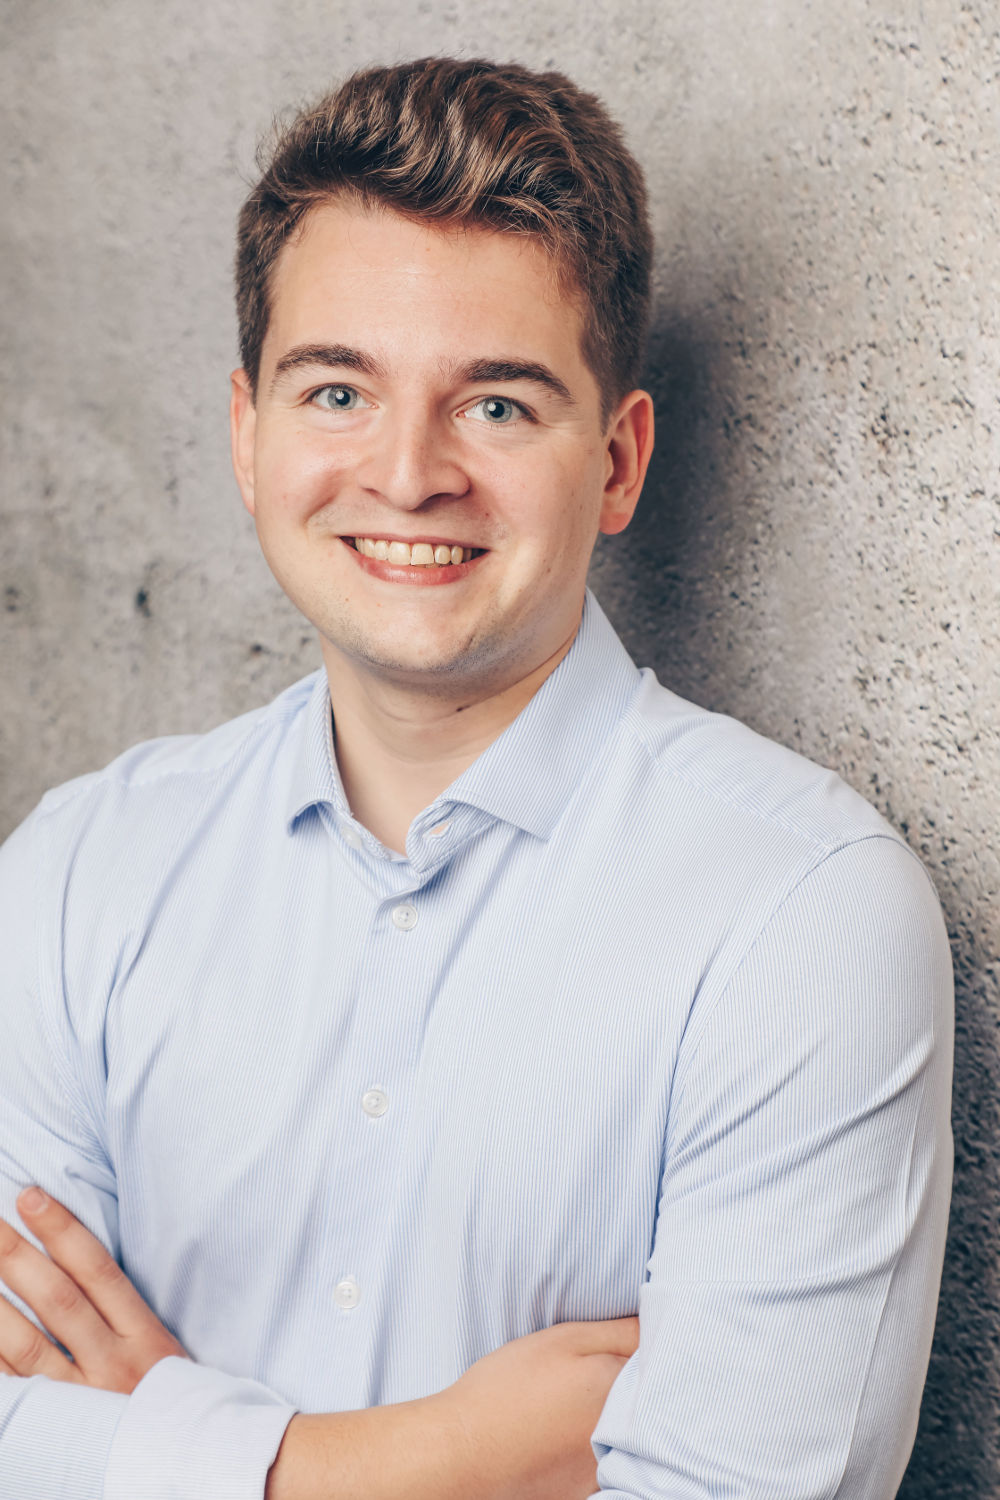
\includegraphics[height=7cm]{oelschlaeger.jpg}
\end{center}

\end{multicols}
\end{adjustwidth}

\vspace{2 mm}
\hrule

%%% Start CV.
\section{Employment}\label{employment}

Research Associate, \emph{Bielefeld University} \hfill 2019 - current

\section{Education}\label{education}

Ph.D.~Student in Econometrics, \emph{Bielefeld University} \hfill 2019 -
current

M.Sc. in Mathematical Economics, \emph{Bielefeld University} \hfill 2017
- 2019

B.Sc. in Mathematics, \emph{Bielefeld University} \hfill 2013 - 2017

\section{Publications}\label{publications}

\subsection{Journal Articles}\label{journal-articles}

\emph{Detecting bearish and bullish markets in financial time series
using hierarchical hidden Markov models}, Oelschläger and Adam (2021),
Statistical Modelling

\subsection{Conference Papers}\label{conference-papers}

\emph{Bayes Estimation of Latent Class Mixed Multinomial Probit Models},
Oelschläger and Bauer (2021), TRB Annual Meeting

\subsection{Software}\label{software}

\href{https://loelschlaeger.de/fHMM/}{fHMM}: Fitting (hierarchical)
hidden Markov models to financial data.

\href{https://loelschlaeger.de/RprobitB/}{RprobitB}: Bayesian estimation
of probit models.

\href{https://loelschlaeger.de/ao/}{ao}: Alternating optimization of
(high-dimensional) functions.

\href{https://loelschlaeger.de/vntrs/}{vntrs}: Variable neighborhood
trust region search.

\href{https://loelschlaeger.de/ino/}{ino}: Initialization of numerical
optimization.

\section{Talks}\label{talks}

Bayes estimation of probit choice models with \{RprobitB\}, \emph{10th
Young Researcher Workshop at Bielefeld University}, 10.03.2022

Klassifizierung von PrC\$ferenzen: Eine Anwendung mit dem R Paket
RprobitB, \emph{27. AKA-Workshop at Kloster Irsee}, 18.11.2021

On the initialization of multinomial probit models, \emph{9th Young
Researcher Workshop at Bielefeld University}, 16.07.2021

Bayes estimation of latent class mixed multinomial probit models,
\emph{Poster Session at the 100th Transportation Research Board Annual
Meeting}, 28.01.2021

Approximating mixing distributions in probit models via a Bayesian
approach, \emph{Centre for Statistics at Bielefeld University},
24.11.2020

Detecting bearish and bullish markets in financial time series using
hierarchical hidden Markov models, \emph{Doctoral Day at Bielefeld
University}, 02.10.2020

\section{Teaching}\label{teaching}

R course, \emph{Bielefeld University} \hfill WT 21/22

Reading course for statistical science, \emph{Bielefeld University}
\hfill WT 21/22

Preparatory course for mathematics, \emph{Bielefeld University}
\hfill WT 21/22

Exercise course for mathematics, \emph{Bielefeld University} \hfill WT
19/20, ST 20, WT 20/21, SS 21, WT 21/22

Tutorial for statistics, \emph{Bielefeld University} \hfill WT 15/16, ST
16, WT 16/17, WT 18/19, ST 19

\section{Miscellanea}\label{miscellanea}

Aviation: I own a private pilot license.

Chess: I play chess since I am 5 years old.

Tennis: Only outside and in good weather.

Languages: English, French, R, LaTeX, Markdown, C++, Matlab, Python,
Java.

\end{document}
